\subsection{TabControl}

\begin{frame}

\begin{CaixaModelo01}{TabControl}
	
	Quando houver muita informação exibida, o controle com abas pode ser útil.
	Pode-se dividi-la em abas.

	\begin{columns}
		\begin{column}{0.48\textwidth}
			\begin{figure}
				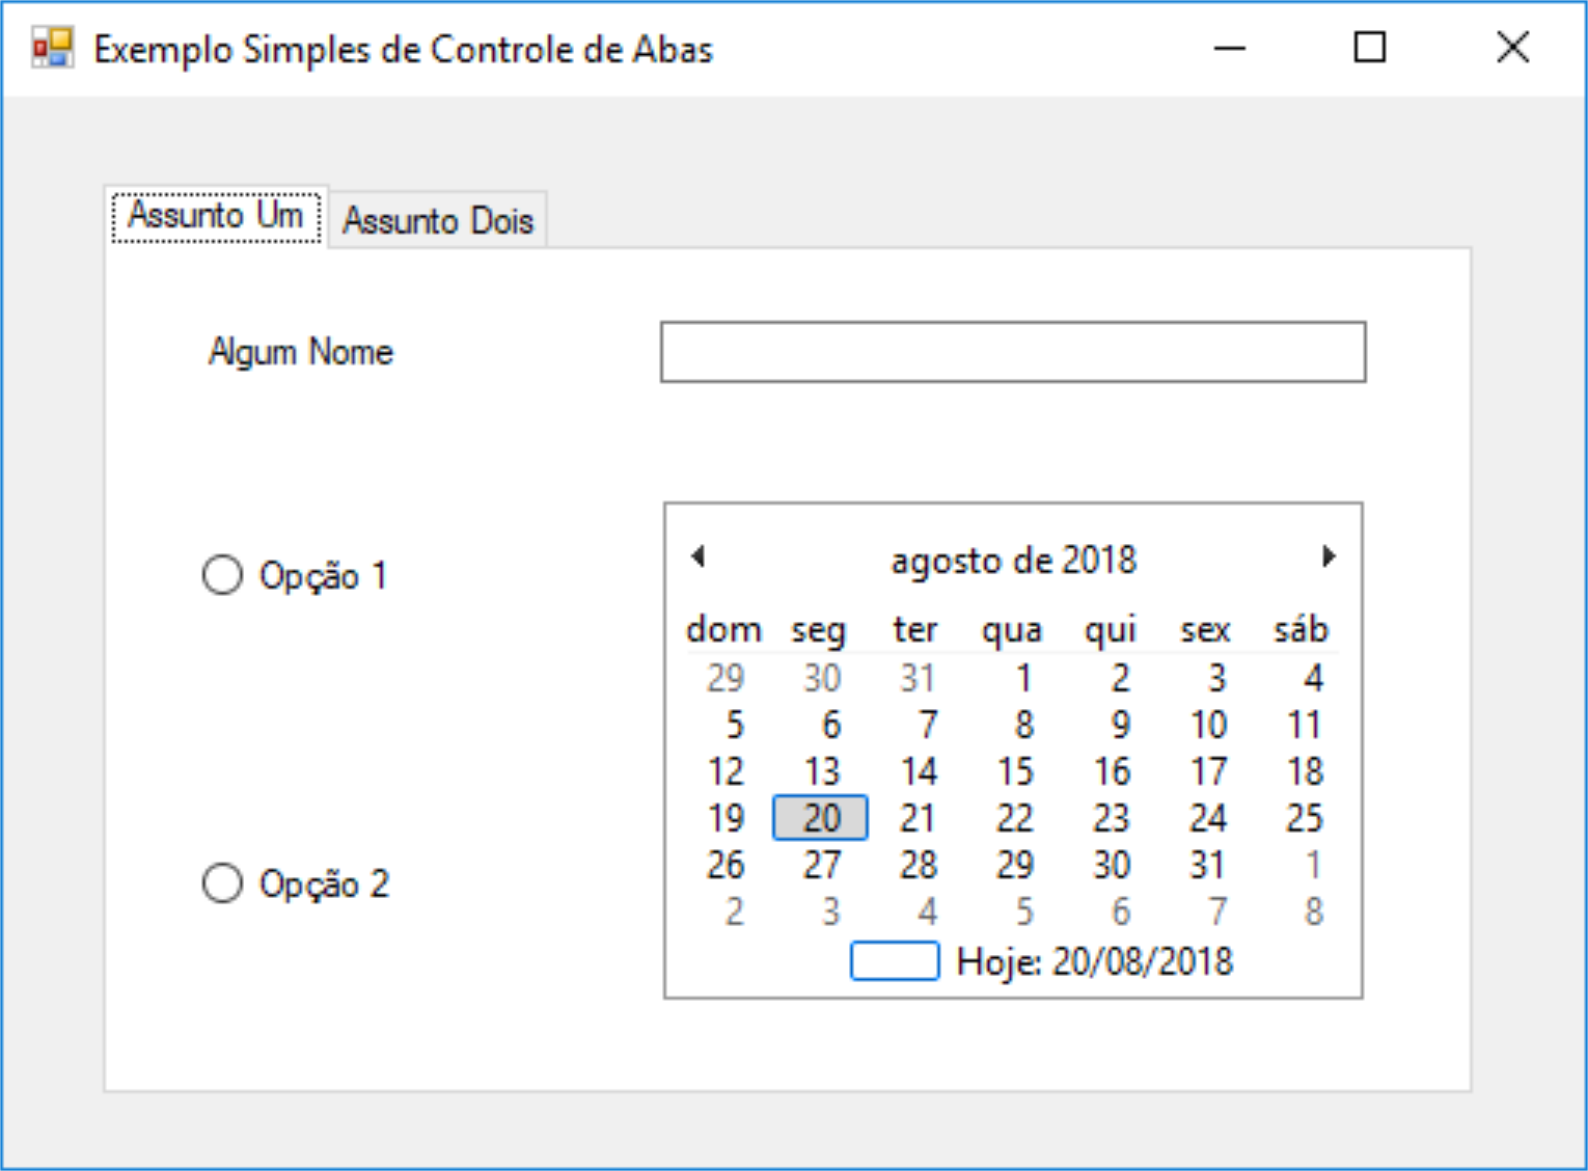
\includegraphics[scale=.35]{./Figuras/F06_Tab01.png}
				\caption{Primeira Aba}
				\label{fig:TabControl01}
			\end{figure}
		\end{column}
		\begin{column}{0.48\textwidth}
			\begin{figure}
				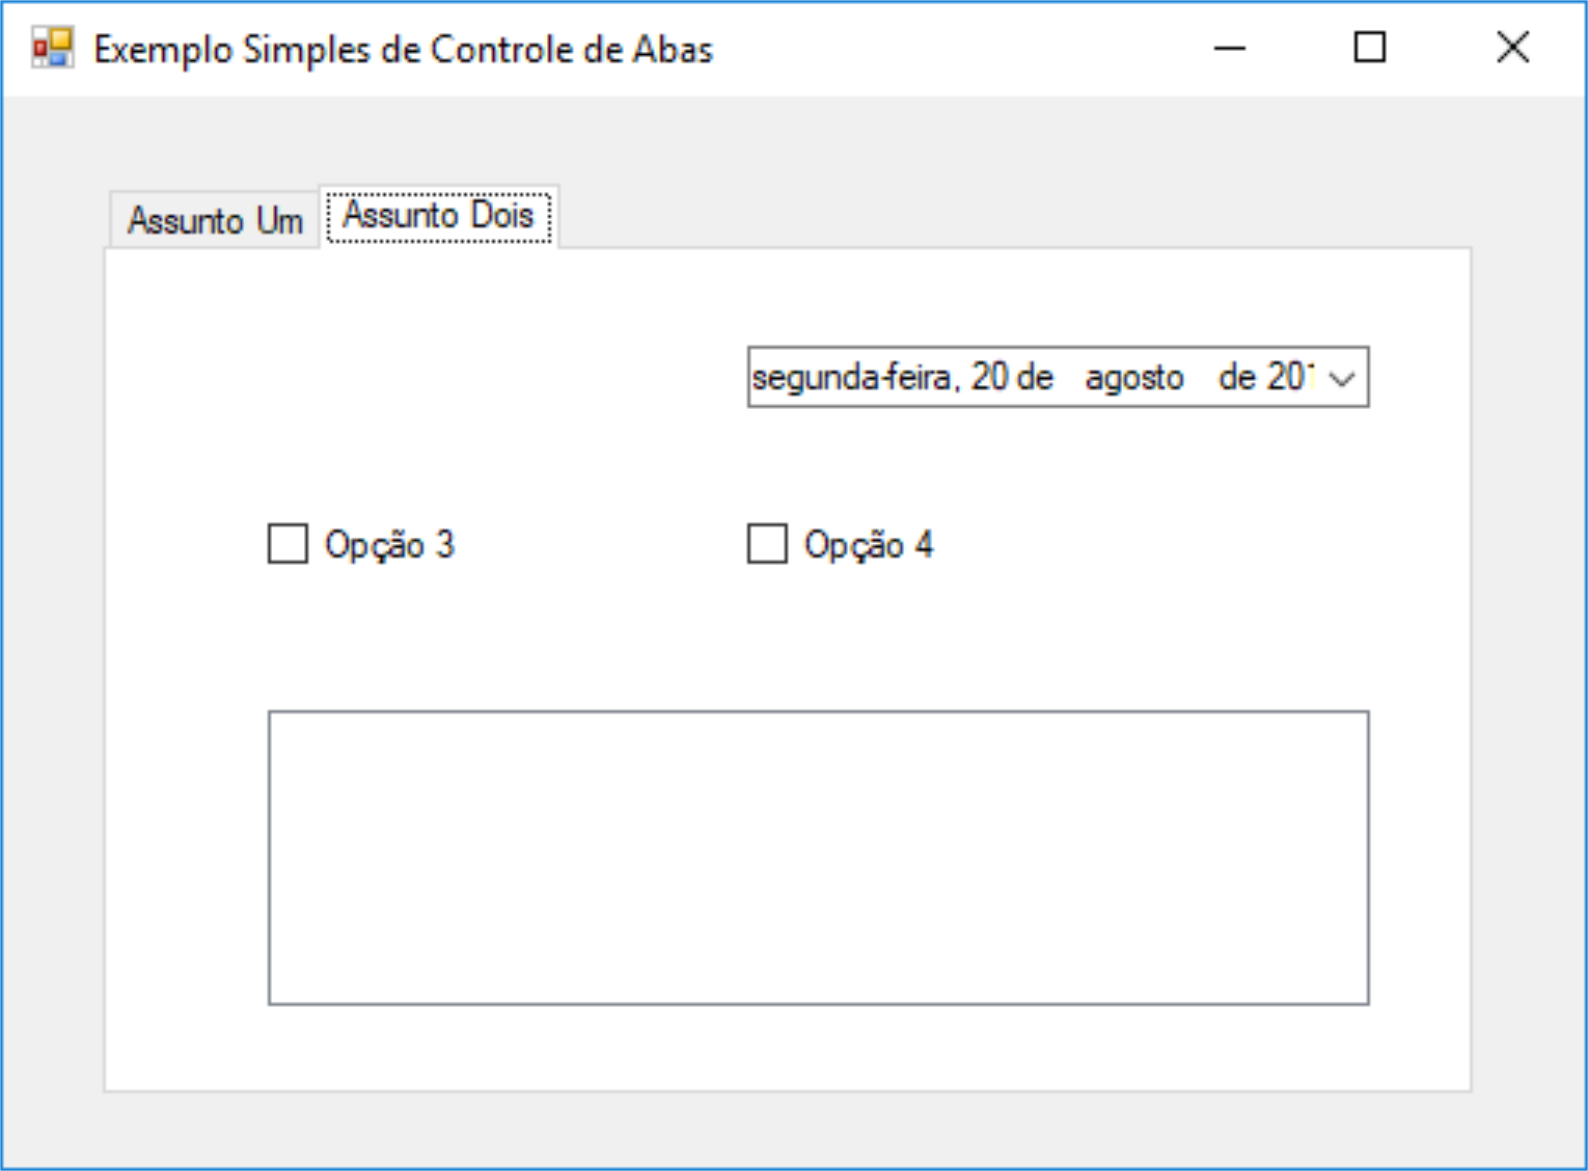
\includegraphics[scale=.35]{./Figuras/F06_Tab02.png}
				\caption{Segunda Aba}
				\label{fig:TabControl02}
			\end{figure}
		\end{column}
	\end{columns}
\end{CaixaModelo01}
\end{frame}
























